% Insert preamble with all the necessary packages.
\RequirePackage[12tabu, orthodox]{nag}

\documentclass[a4paper]{article}
\usepackage[english]{babel}
\usepackage[utf8]{inputenc}
\usepackage{minted}
\usepackage{textcomp}
\usepackage{amsmath}
\usepackage{nameref}
\usepackage{enumitem}
\usepackage{url}
\usepackage{graphicx}
\usepackage{caption}
\usepackage{subcaption}
\usepackage{tikz-qtree}
\usepackage{listings}
\usepackage{amsmath}
\usepackage{amssymb}
\usepackage{color}
\usepackage{microtype}
\usepackage{siunitx}
\usepackage{booktabs}
\usepackage[colorlinks=false, pdfborder={0 0 0}]{hyperref}
\usepackage{cleveref}
\usepackage{color}
\usepackage[tableaux]{prooftrees}
\usepackage[total={6.7in,10.2in}, % text area width and height
		    top=1in, left=1in, right=1in, bottom=1in,% top and left margin
		    includefoot]{geometry}
\renewcommand*\linenumberstyle[1]{(#1)}


\definecolor{mygreen}{rgb}{0,0.6,0}
\definecolor{mygray}{rgb}{0.5,0.5,0.5}
\definecolor{mymauve}{rgb}{0.58,0,0.82}

\lstset{ %
  backgroundcolor=\color{white},   % choose the background color; you must add \usepackage{color} or \usepackage{xcolor}
  basicstyle=\footnotesize\ttfamily,       % the size of the fonts that are used for the code
  breakatwhitespace=false,         % sets if automatic breaks should only happen at whitespace
  breaklines=true,                 % sets automatic line breaking
  captionpos=b,                    % sets the caption-position to bottom
  commentstyle=\color{mygreen},    % comment style
  deletekeywords={...},            % if you want to delete keywords from the given language
  escapeinside={\%*}{*)},          % if you want to add LaTeX within your code
  extendedchars=true,              % lets you use non-ASCII characters; for 8-bits encodings only, does not work with UTF-8
  frame=l,                    % adds a frame around the code
  keepspaces=true,                 % keeps spaces in text, useful for keeping indentation of code (possibly needs columns=flexible)
  keywordstyle=\color{blue},       % keyword style
  language=Java,                   % the language of the code
  morekeywords={*,...},            % if you want to add more keywords to the set
  numbers=left,                    % where to put the line-numbers; possible values are (none, left, right)
  numbersep=8pt,                   % how far the line-numbers are from the code
  numberstyle=\tiny\color{mygray}, % the style that is used for the line-numbers
  rulecolor=\color{black},         % if not set, the frame-color may be changed on line-breaks within not-black text (e.g. comments (green here))
  showspaces=false,                % show spaces everywhere adding particular underscores; it overrides 'showstringspaces'
  showstringspaces=false,          % underline spaces within strings only
  showtabs=false,                  % show tabs within strings adding particular underscores
  stepnumber=1,                    % the step between two line-numbers. If it's 1, each line will be numbered
  stringstyle=\color{mymauve},     % string literal style
  tabsize=2,                       % sets default tabsize to 2 spaces
  title=\lstname                   % show the filename of files included with \lstinputlisting; also try caption instead of title
}

%Code for DTU logo as background picture.
\usepackage{eso-pic}
\newcommand\BackgroundPic{%
\put(10,5){%
\parbox[b][13cm]{32cm}{%
\vfill
\centering

\includegraphics[width=6cm,height=\paperheight,%
keepaspectratio]{./Output/DTU.jpg}%
\vfill
}}}

\begin{document}

% Insert frontpage
%----------------------------------------------------------------------------------------
%	TITLE SECTION
%----------------------------------------------------------------------------------------

\title{\vspace{-15mm}\fontsize{24pt}{10pt}\selectfont\textbf{Pommerman}} % Article title

\author{
\large
\textsc{Alexander D Juhl, Marc S. Larsen, Marcus Skov Hansen} \\ 
\textsc{Mark B. Jensen, Mathias P. V. Mortensen}\\[2mm]%\thanks{A thank you or further information}\\[2mm] % Your name
\normalsize Department of Applied Mathematics and Computer Science,\\
\normalsize Technical University of Denmark, 2800 Kgs. Lyngby, Denmark \\ % Your institution
%\normalsize \href{mailto:john@smith.com}{john@smith.com} % Your email address
\vspace{-5mm}
}
\date{}

%----------------------------------------------------------------------------------------

\maketitle % Insert title

\thispagestyle{fancy} % All pages have headers and footers

\begin{onecolabstract}
\noindent 
\end{onecolabstract}

% Two-column layout throughout the main article text
\begin{multicols}{2}

% Sections of the main article.
\section{Introduction}
\label{sec:intro}
% MAKE IT VERY CLEAR THAT WE WANT TO RESEARCH EASIER METHODS THAN ACTOR CRITIC FOR SOLVING THE PROBLEM

% Reinforcement learning has previously been used to solve a number of different games such as Chess\footnote{\href{https://arxiv.org/pdf/1712.01815.pdf}{Mastering Chess and Shogi by Self-Play with a General Reinforcement Learning Algorithm}} and Go\footnote{\href{https://www.nature.com/articles/nature24270.epdf}{Mastering the game of Go without human knowledge}}, both of which are zero sum games. Reinforcement learning has excelled at playing Go, where the number of possible moves are so many that a traditional heuristic is not sufficient to solve the problem successfully. These games only contain two players, whereas a game like Dota II is 5 vs. 5 game. That makes it a multi-agent environment and a non-zero sum game, which introduces additional challenges for machine learning.\footnote{\href{https://blog.openai.com/openai-five/}{OpenAI Five}}

\emph{\say{Accomplishing tasks with infinitely meaningful variation is common in the real world and difficult to simulate.}}\cite{pommerman} One place where this can be simulated is in games. Reinforcement learning has in recent years been utilised to solve a number of games such as Go\cite{silver2017masteringgo}\cite{silver2016a}, chess\cite{silver2017masteringchess} and many others\cite{mnih2015a}. In the game of Go does the number of possible moves by far exceeds the capabilities of a traditional heuristic, but reinforcement learning has shown to be excellent for training an agent to solve the problem of playing and winning the game successfully.\cite{silver2017masteringgo} The huge amount of unique states in Go is similar to the game of Pommerman, which is a variation of the original Bomberman developed by Hudson soft. in 1983. In Pommerman is every game played on a new random generated board, as seen in figure~\ref{fig:pomIntro} and the game can be played as a Free For All (FFA) or as in teams of two.\cite{pommerman} The random boards and the four players moving independently of each other are the reasons for the vast number of possible states in the game.

\begin{figure}[htb]
    \centerline{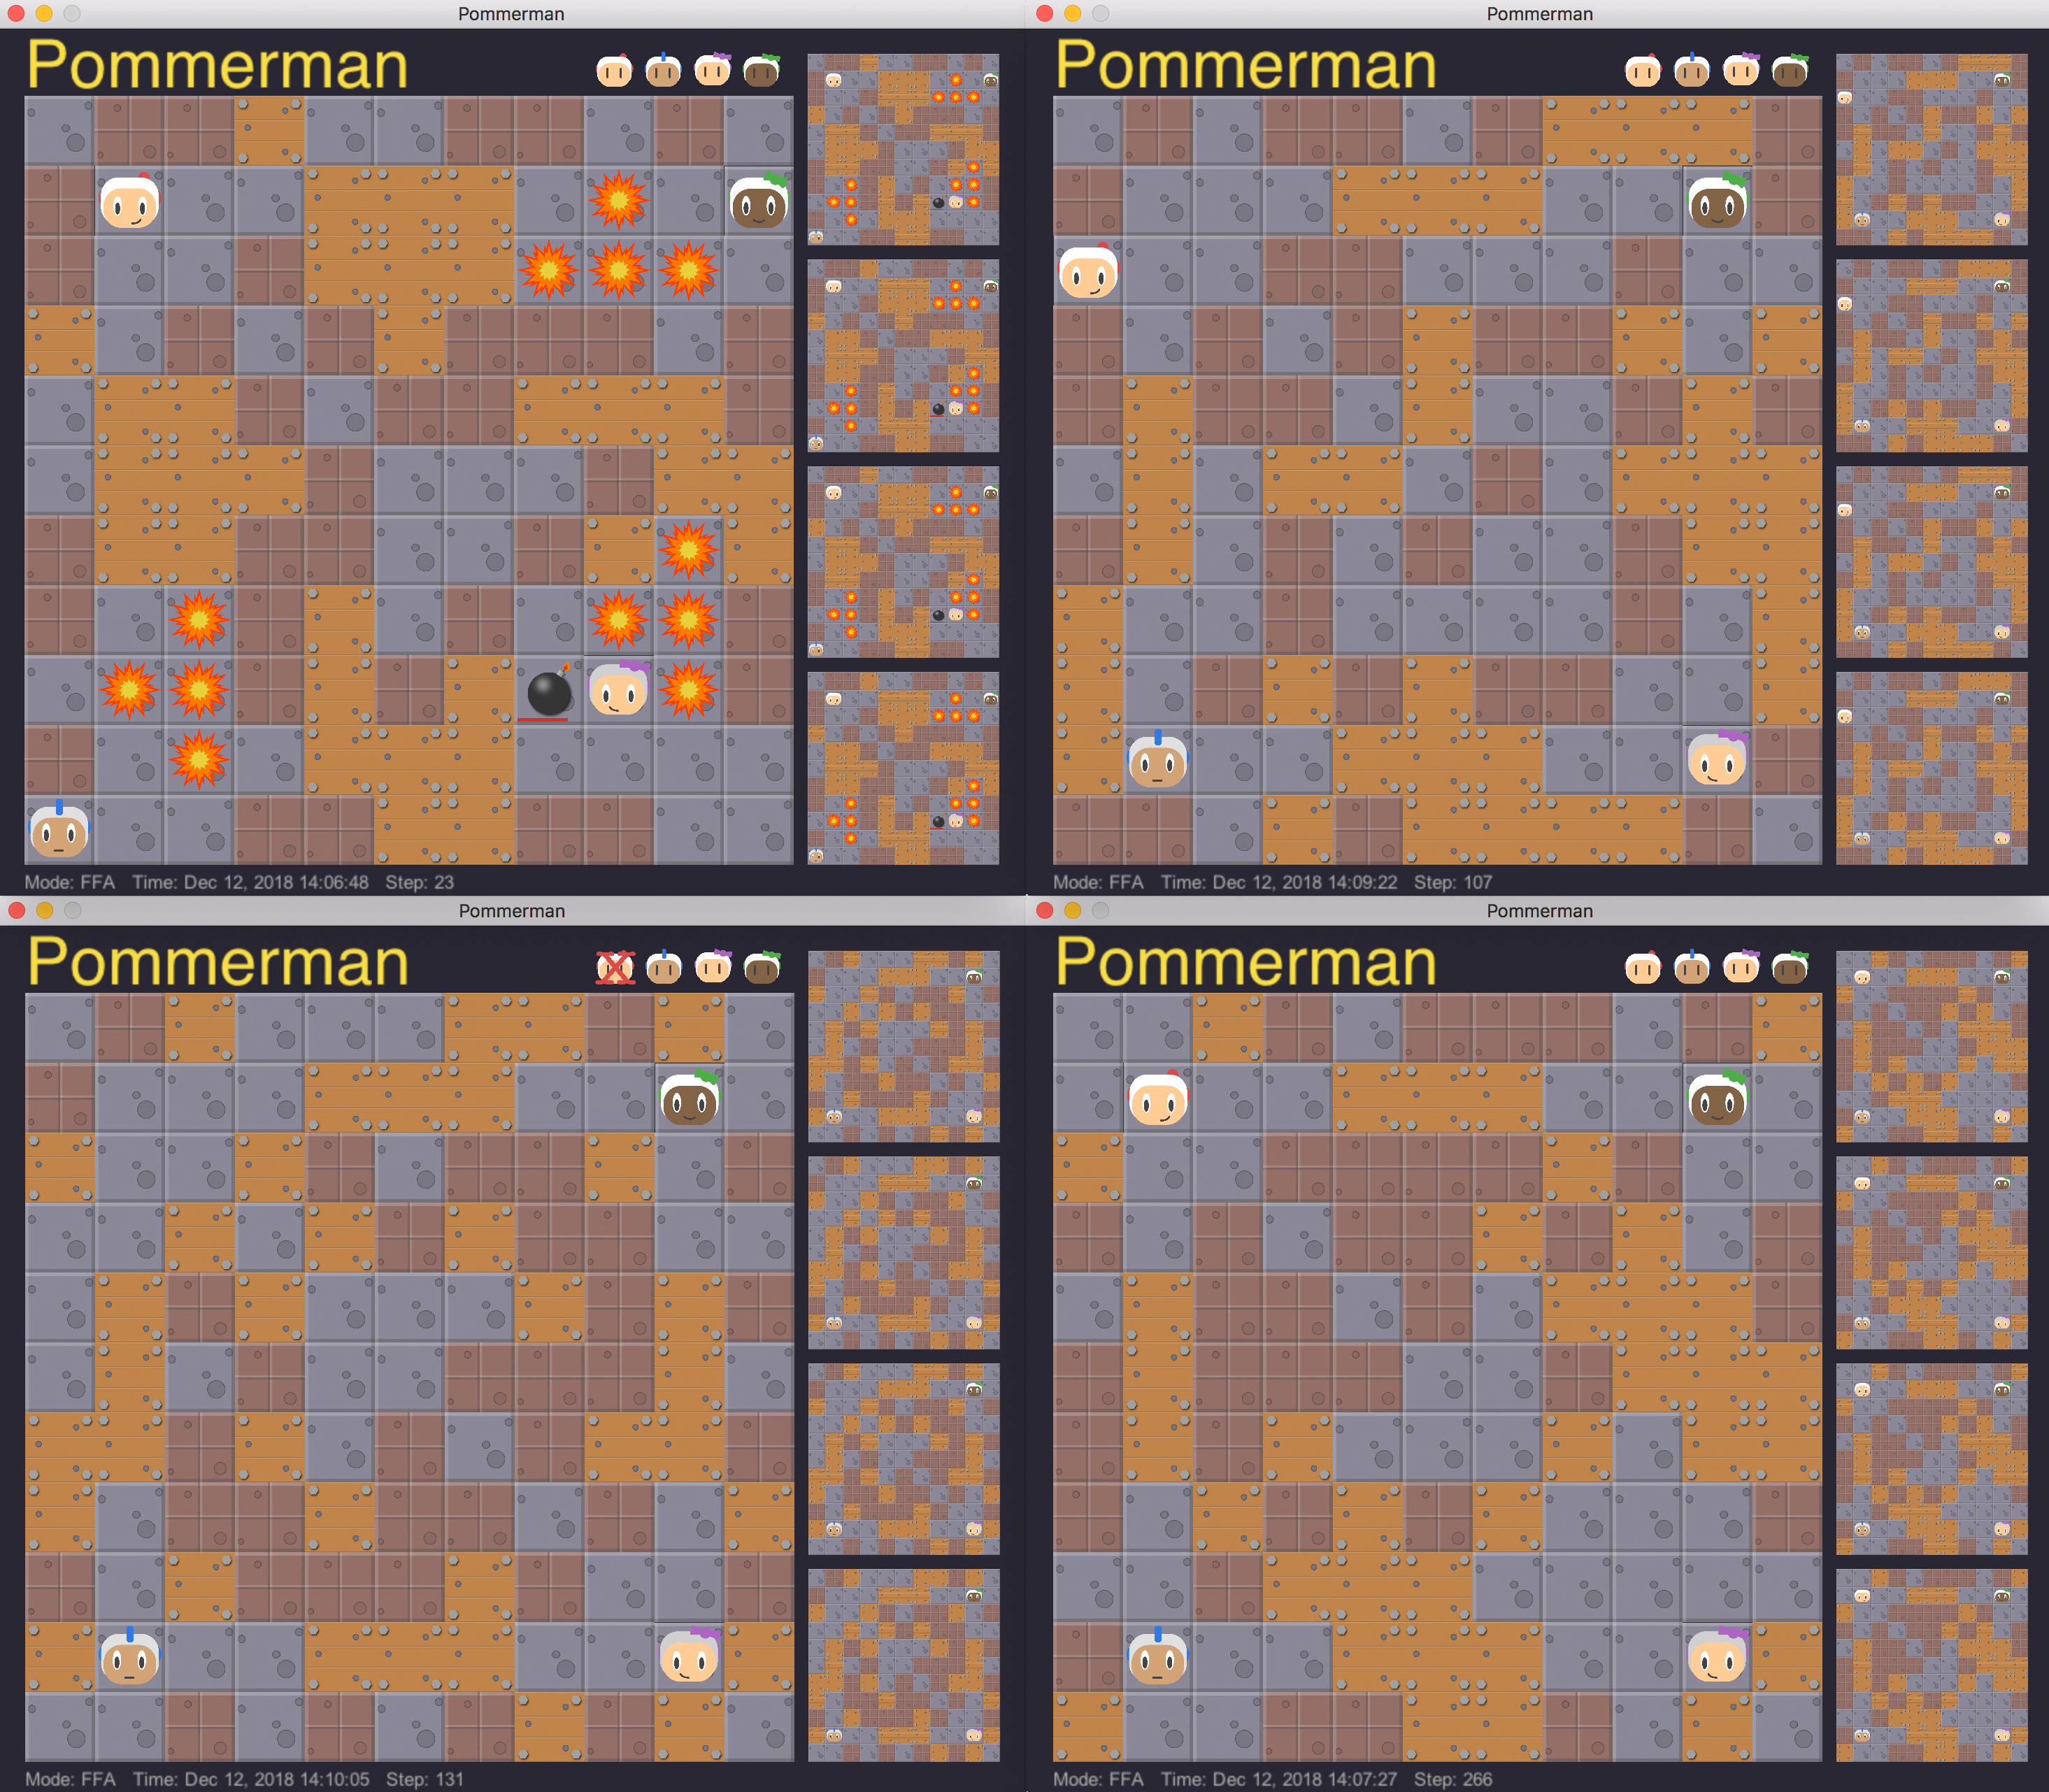
\includegraphics[width=0.7\linewidth]{docs/article/inputs/4pommerview.jpg}}
    \caption{Four random boards in typical games of Pommerman.}
    \label{fig:pomIntro}
\end{figure}

In the FFA version of Pommerman has the actor-critic algorithm shown to be performing very well.\cite{rwightman} The goal in this paper is to research if other more simple deep reinforcement learning algorithms can be utilised to solve the problem of training an agent to play the FFA Pommerman against so called random and simple agents, with similar or better performance than what is the result of \cite{rwightman}. The motivation for doing so... INSERT MOTIVATION HERE

% Motivation
% The motivation for researching state of the art techniques for solving these problems is intriguing. Although much research has been done in the past years we have not yet seen revolutionary approaches, making headline such as AlphaZero or AlphaGo. We as a group would like to explore these state of the art approaches on the game Pommerman to evaluate how far machine learning has come, solving non-zero sum games in single- and multi-agent environments. We do not strafe for ground breaking research within the topic.

% Give an overview of the article, section by section
In section~\ref{sec:relatedwork}, are related works presented. In section~\ref{sec:methods} are the different algorithms described as well as implemented features to restrict the complexity of the problem and increase the performance of the agent. In section~\ref{sec:results} are the results of the implements methods shown. In section~\ref{sec:discussion} are the issues faced during the research discussed. In section~\ref{sec:futurework} will it be covered what techniques and algorithms should be investigated in future work. Finally is the paper concluded in section~\ref{sec:conclusion}.

% Basically knowledge needed to understand the article. Here could be things from the book if we deem it needed (maybe ask monday?)
\section{Background}

% Related work is other articles and solutions. Can often be in introduction or background if we want.
\section{Related Work}
% Related work is other articles and solutions. Can often be in introduction or background if we want.
% - Starting point

% Questions to answer for each source
% - What problem do they solve?
% - How do they solve it?
% - How does it relate to Pommerman?


% https://github.com/rwightman/pytorch-pommerman-rl
\subsection{PyTorch RL for Pommerman}

% http://www.ai.rug.nl/~mwiering/GROUP/ARTICLES/ICAART_EXPLORATION_BOMBERMAN_2018.pdf
\subsection{Exploration Methods for Connectionist Q-Learning in Bomberman}

% https://cs.gmu.edu/~eclab/papers/panait05cooperative.pdf
\subsection{Cooperative Multi-Agent Learning: The State of the Art}

% https://arxiv.org/pdf/1706.02275.pdf
\subsection{Multi-Agent Actor-Critic for Mixed Cooperative-Competitive Environments}

% Sometimes mentioned as experiments/results. Maybe experiments sounds better for us xD
\section{Results}
\label{sec:results}
% Mention stop agents

The results were collected by training and validating the agent against three opponents at the same time of the same type. During training and validation primarily two types of agents were used, namely the random and simple agents from the Pommerman environment used. Occasionally was our stop agent used as well.

The first model that was trained was utilising the REINFORCE algorithm, see section~\ref{sec:reinforce}, our convolutional network, see section~\ref{sec:conv}, the $\epsilon$-greedy strategy with decay, see figure~\ref{fig:gamma}(a), a static board, see section~\ref{sec:static}, and finally the standard reward function of $-1$ for a loss and $1$ for a win. In figure~\ref{fig:resultsrandom} the validation and training error of the agent trained against three random agents is displayed. Remember that with the $\gamma$ function used for the $\epsilon$-greedy strategy the agent will keep exploring until approximately $85\%$ of the iterations has been played. From figure~\ref{fig:resultsrandom} one can see that around the $85\%$ mark the validation and training rewards are both $1.00$, but already from the first validation is the agent achieving a reward of $1$. Looking at the actions the agent were performing, it is clear to see that the agents has learning to perform any single action that is not placing a bomb, thereby waiting for the random agents to kill themselves and winning the game.

\begin{figure}[htb]
    \centerline{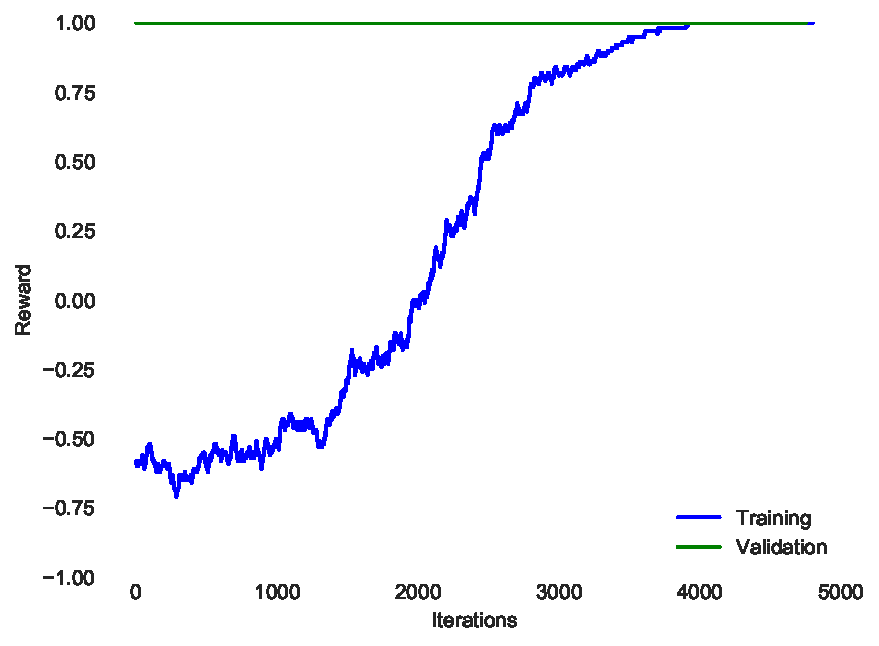
\includegraphics[width=1.0\linewidth]{pommerman/plots/random_train_val.pdf}}
    \caption{Moving average of validation and training rewards against random agents.}\label{fig:resultsrandom}
\end{figure}

In figure~\ref{fig:resultssimple} the validation and training rewards of the agent trained against three simple agents are displayed, using the same model as against the three random agents. From figure~\ref{fig:resultssimple} it is seen that there is a slight incline in the training reward as the agent starts to exploit more and more. However, it does seem to flatten a bit towards the last 5000 iterations. The incline is due to the simple agents are killing each other and themselves without our agent killing itself, thereby never reaching our agent and leaving it to win and receive a reward of $1$. Looking at the reward for the validation it seems to be moving around an average of $-0.65$, with a slight incline in the reward towards the end of the training of the agent.

\begin{figure}[htb]
    \centerline{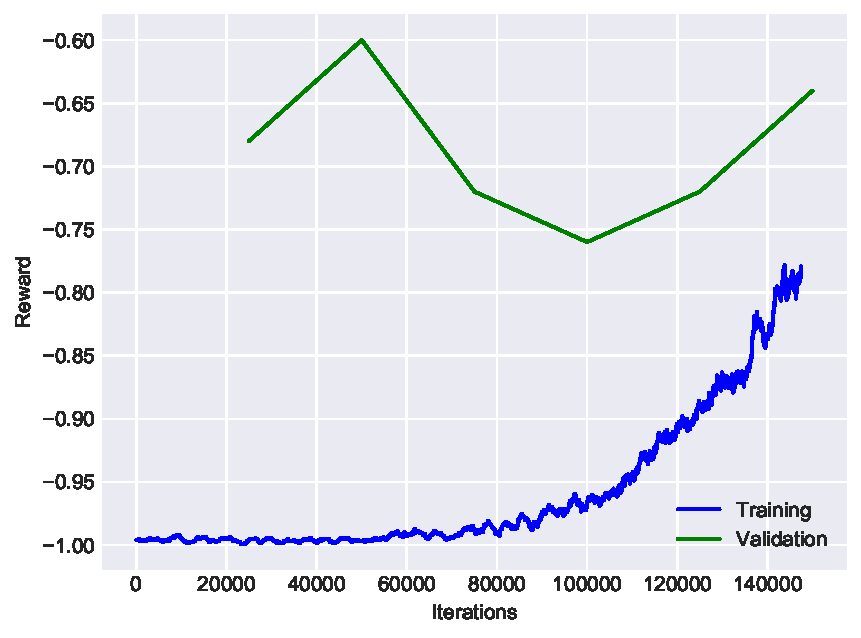
\includegraphics[width=1.0\linewidth]{pommerman/plots/train_val.pdf}}
    \caption{Moving average of validation and training rewards against simple agents.}\label{fig:resultssimple}
\end{figure}

The probabilities of each action during the training against the three simple agents can be seen in figure~\ref{fig:act}. From this it is evident that the probability of the two actions \emph{Down} and \emph{Right} are in a constant incline, the probability for \emph{Bomb} is on a constant decline and the remaining actions are fairly stable until the \nth{105000} iteration. After that the probability of the action \emph{Down} increases extremely fast towards $1$ and the remaining probabilities decreases towards $0$. Now that it is clear that the agent is performing a single action towards the end of where it fully exploits, the incline in its training and validation rewards is purely because of the actions of the other agents. Had the agent been run for more iterations where it would fully exploit, it would most likely be the case that the two rewards would go towards each other and be stationary around the same reward.

\begin{figure}[htb]
    \centerline{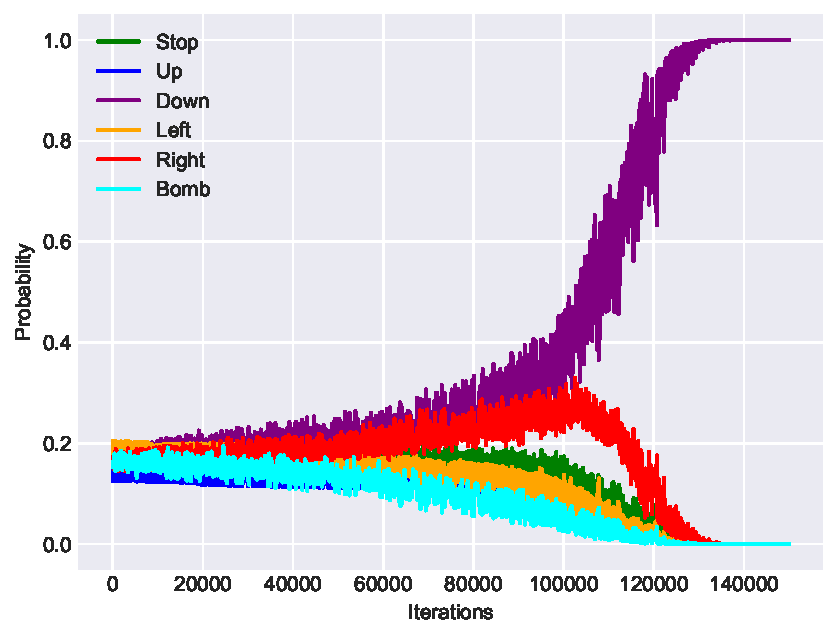
\includegraphics[width=1.0\linewidth]{pommerman/plots/a_probs.pdf}}
    \caption{Distribution of action probabilities.}\label{fig:act}
\end{figure}

% THIS HAS TO BE ADJUSTED IF WE ADD THE RESULT OF THE MODEL USING THE CUSTOM REWARD FUNCTION.
It should be emphasised that despite only showing the results of one model, the agent has been trained with numerous different models. The models have had its hyper parameters changes, different networks and sizes and reward functions. Furthermore have they been trained against the standard dynamic boards and our custom static board. Each configuration has been run for $150.000$ games. However, despite these different configurations all networks ended up producing the near same rewards results and converged towards picking one action, as was the case shown in figure~\ref{fig:act}. This also turned out to be independent of whether REINFORCE or Q-learning was used.

% Sometimes mentioned as experiments/results. Maybe experiments sounds better for us xD
% Show that the agent was able to learn playing against 3 random agents
% Show graphs for result for playing against 3 simple agents (-1 constantly, easy graph)

%\subsection{Performance}
% As in iterations, training time etc.
% Mention the number of iterations 

% Result for every method used should be stated

\section{Discussion}
\label{sec:discussion}

\subsection{Reward function}

\subsection{Lack of training}
% - Complexity
%   - It takes a lot of correct random actions to get a reward of 1 by killing the enemies
% - Exploration / Exploitation
It is evident from the literature that all the agents that do well have been trained for millions of times. An example of this is \cite{rwightman}'s agent, which has been trained for the same pommerman environment for approximately 60 millions games. Another one is \cite{kormelink2018exploration} which has been trained for a million games, but in a $7 \times 7$ static classic bomberman environment rather than a $11 \times 11$ environment. All of the trained setups showed the same sign of early convergence towards a single action. Our hypothesis is that the setups simple have not had enough time for training and a lot more training would yield for more exploration in the massive search space. This could result in that the agent would be able to take more meaningful actions rather than just sticking to a single action. The reasoning behind this hypothesi



Problems in learning to play could be because of the gap between an untrained agent and the actions needed to beat three simple agents is simply too large. That gab combined with the ever changing board and the randomness in the simple agents movement would create a giant search space and likely result in the agent never learning why it lost the game.


\subsection{Networks}

% "Derp train more". Could be in discussion maybe?
\section{Future Work}
% "Derp train more". Could be in discussion maybe?
% Actor critic

% Maybe not necessary if we have both results and discussion.
\section{Conclusion}
\label{sec:conclusion}

%\begin{thebibliography}{9} % Bibliography - this is intentionally simple in this template

\bibitem[Bondy et al, 1976]{BondyMurty:1976}
    Bondy, J.~A. and Murty, U.~S.~R (1976).
    \newblock Graph Theory With Applications,
    \newblock ch. 1-2,
    \newblock 1. Edition,
    \newblock The Macmillan Press Ltd., Great Britain
    
\bibitem[Corey et al, 1995]{Corey:1995}
    Corey, E.~J. and Cheng X-M. (1995).
    \newblock The Logic of Chemical Synthesis,
    \newblock 1. Edition,
    \newblock Wiley-Interscience, New York.
    
\bibitem[Cormen et al, 2009]{Cormen:2009}
    Cormen, T.~H.; Leiserson, C.~E.; Rivest, R.~L. and Stein, C. (2009).
    \newblock Introduction to Algorithms,
    \newblock ch. B.5,
    \newblock 3. Edition,
    \newblock The MIT Press, Cambridge, Massachusetts.

\bibitem[May et al, 1976]{MayRudd:1976}
    May, D. and Rudd, D.~F. (1976).
    \newblock Development of Solvay Clusters of Chemical Reactions,
    \newblock {\em Chemical Engineering Science}, 31:59--69,
    \newblock Pergamon Press, Great Britain.

\bibitem[Nilsson, 2012]{Nilsson:2012}
    Nilsson, J.~F. (2012).
    \newblock Computerized Means-End Reasoning Applied to Chemical Retro-Synthesis,
    \newblock {\url{www.campusnet.dtu.dk}}
    
\bibitem[NIOSH, 2014]{NIOSH:2014}
    \newblock Hydrogen chloride,
    \newblock{\url{http://www.cdc.gov}},
    \newblock 4$^{th}$ December 2014.
    \newblock{\url{http://www.cdc.gov/niosh/idlh/7647010.html}},
    \newblock (Retrieved: 16$^{th}$ June 2016).

\bibitem[Rudd, 1976]{Rudd:1976}
    Rudd, D.~F. (1976).
    \newblock Accessible Designs in Solvay Cluster Synthesis,
    \newblock {\em Chemical Engineering Science}, 31:701--703,
    \newblock Pergamon Press, Great Britain.

\bibitem[Russell et al, 1995]{RussellNorvig:1995}
    Russell, S. and Norvig, P. (1995).
    \newblock Artificial Intelligence A Modern Approach,
    \newblock ch. 3,
    \newblock 3. Edition,
    \newblock Pearson Education, Inc., United States of America.

\bibitem[Wikipedia, 2016]{Wiki:2016}
    \newblock Reaction scheme of the Leblanc process,
    \newblock {\url{https://en.wikipedia.org/wiki/Leblanc_process}},
    \newblock 17$^{th}$ January 2016.
    \newblock {\url{https://en.wikipedia.org/wiki/Leblanc_process#/media/File:Leblanc_process_reaction_scheme.svg}},
    \newblock (Retrieved: 13$^{th}$ April 2016).
\end{thebibliography}
\bibliographystyle{lnig}
\bibliography{sections/bibliography}

% End the two-column layout from the main article text
\end{multicols}

% Makes sure that there's a pagebreak before the appendix.
\pagebreak

\section*{Appendix}
\appendix
The program has been structured such that one can easily swap different components, like the network, algorithm or opponents to train against. This modular structure of the program can be seen in figure~\ref{fig:uml}.
\begin{figure}[htb]
    \centerline{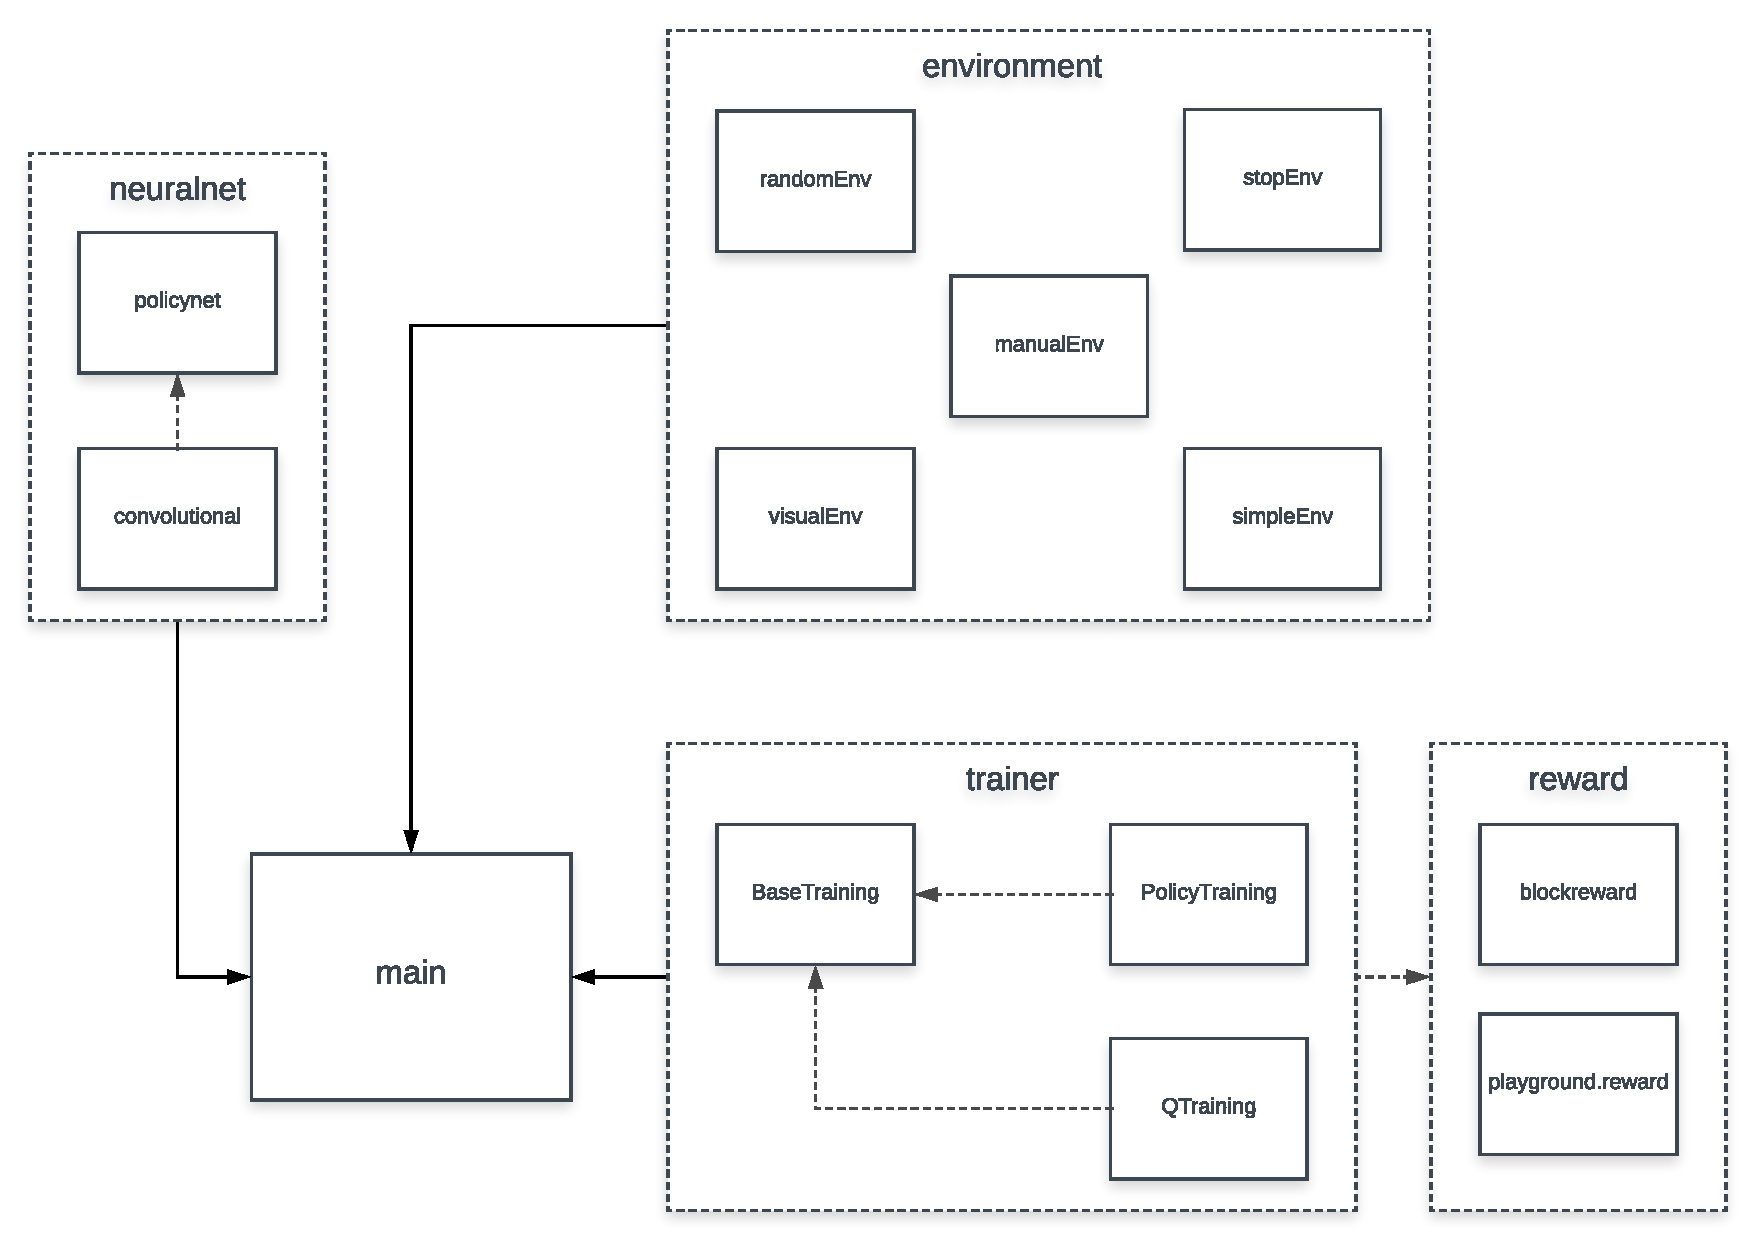
\includegraphics[width=0.8\linewidth]{docs/article/inputs/02456-UML.pdf}}
    \caption{UML of workflow.}\label{fig:uml}
\end{figure}


\end{document}